\apendice{Plan de Proyecto Software}

\section{Introducción}

En este apartado se va a detallar como se ha llevado a acabo la planificación del proyecto. En la planificación es donde se estudia el coste tanto en tiempo, como en recursos y también, aunque sea un proyecto educacional, el coste económico y sus posibles beneficios.

Con los resultados obtenidos realizaremos la planificación temporal del proyecto y el estudio de viabilidad del mismo. 

\section{Planificación temporal}

Como ya se ha mencionado en el inicio del proyecto se ha optado por seguir la metodología ágil \emph{Scrum}. Se ha intentado seguir fielmente, con la salvedad de que normalmente en este tipo de proyectos participan varias personas y en este ha participado solo una persona, con la supervisión del tutor.

\begin{figure}[H]
	\centering
	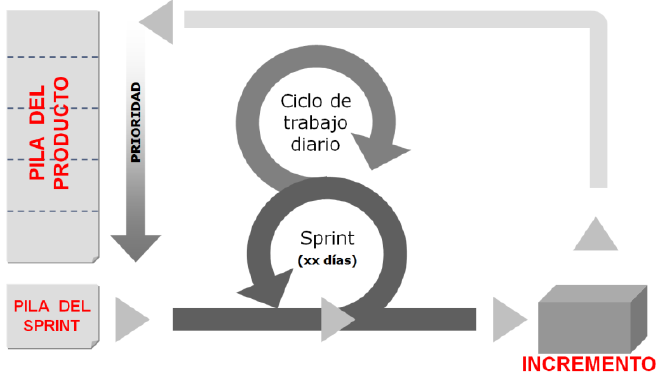
\includegraphics[width=0.7\textwidth]{Scrum}
	\caption{Diagrama del ciclo iterativo \emph{Scrum}.}
	\label{fig:Scrum}
\end{figure}

\emph{Scrum} se basa en aplicar una estrategia de desarrollo incremental, que intenta mantener un ritmo de avance constante. Se planifican una serie de \emph{sprints} donde se debían desarrollar una serie de tareas completamente funcionales. La duración de estos \emph{sprints} era de una semana y al final de cada \emph{sprint} se realizaban reuniones para comprobar si se habían cumplido los objetivos y planificar el siguiente \emph{sprint}.

Los requisitos del sistema se registraron en dos formatos:

\begin{itemize}
\item \textbf{Pila del producto:} como una  lista ordenada de todo aquello que el propietario de producto cree que necesita el producto. La pila del producto nunca se da por completada; está en continuo crecimiento y evolución.

\item \textbf{Pila del \emph{sprint}:} como una lista de las tareas necesarias para construir las historias de usuario que se van a realizar en un \emph{sprint}. Refleja los requisitos vistos desde el punto de vista del equipo de desarrollo.
 
\end{itemize}

Para la gestión del proyecto se utilizó \emph{ZenHub}, en ella podíamos hacer el seguimiento de lo que está en revisión, lo que debe probarse, lo que se está haciendo o lo ya cerrado.


\begin{figure}[H]
	\centering
	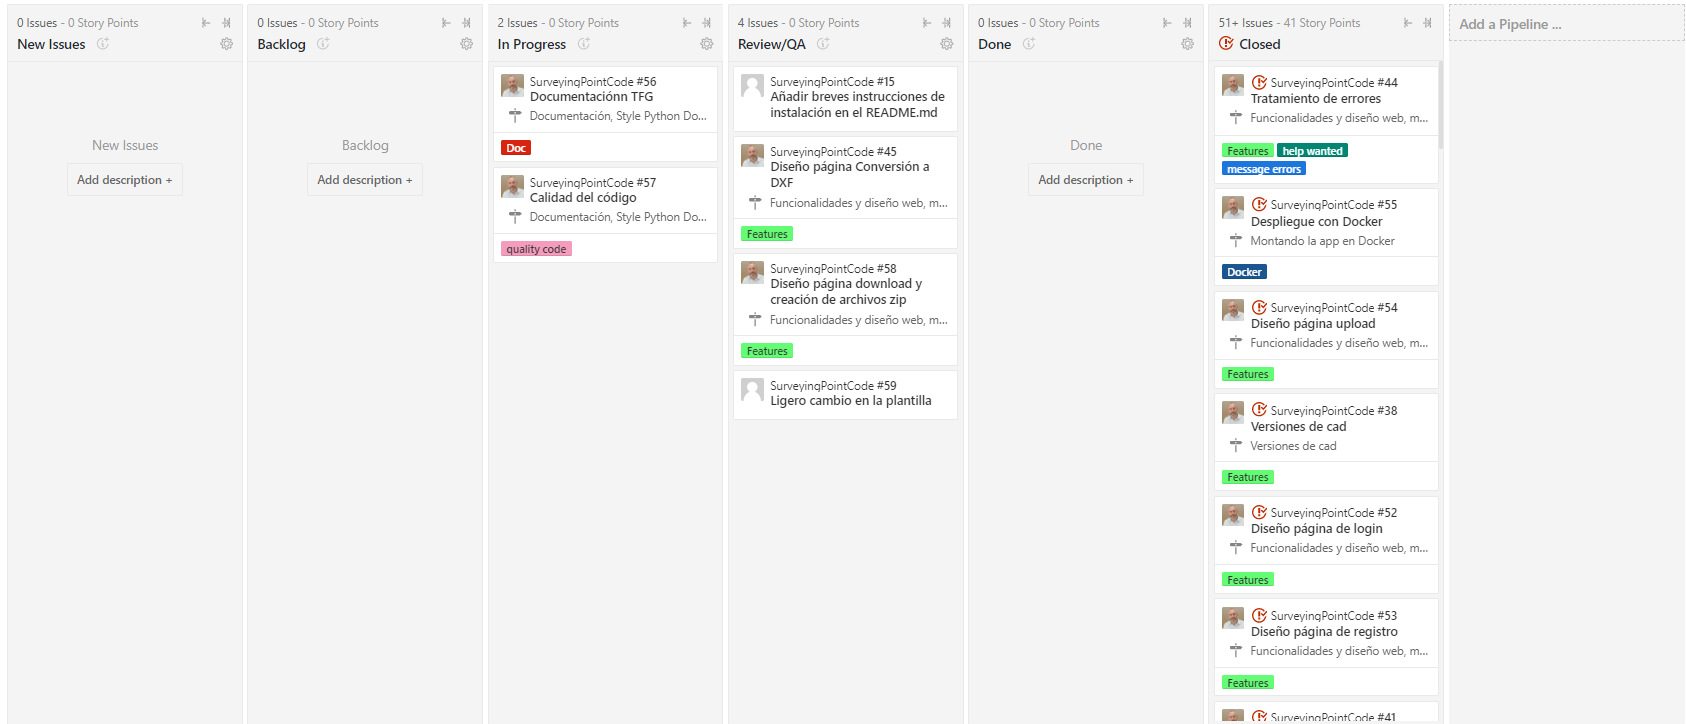
\includegraphics[width=0.9\textwidth]{ZenHub}
	\caption{Gestión de tareas con \emph{ZenHub} en una fase del proyecto.}
	\label{fig:ZenHub}
\end{figure}

A continuación se describen los diferentes \emph{sprints} que se han realizado:

\subsection{\emph{Sprint} 1 (24/01/2019 - 30/01/2019)}

En este primer \emph{sprint} y como primera toma de contacto con el proyecto, los objetivos planteados fueron los siguientes:

\begin{itemize}
\item Preparación del entorno de trabajo. El proyecto se iba a desarrollar en Python, se instaló la version \emph{Python 3.7} y como entorno de  la aplicación \emph{PyCharm 2019.1.1 Comunity Edition}.

\item Repaso de conocimientos en \emph{GIT} y creación del repositorio en \emph{GitHub}. Se refrescaron los conocimientos en \emph{GIT}, en algunos tutoriales  online como  \textit{git - la guía sencilla} \cite{git} y \textit{Tutorial de Git. Manual básico con ejemplos} \cite{git_1}

\item Formación en \emph{PEPs}. Para conocer bien las guías de estilo y la convenciones de \emph{Python}, se consultaron las guías PEP 8 y PEP 257, mencionadas en la memoria.

\item Formación en \LaTeX. Se consulto como guía principal, el libro Edición de Textos Científicos LaTEX\cite{latex}. Y como herramientas para realizar la memoria se instalaron las aplicaciones :\emph{Texmaker 5.0.3} y \emph{MikTex 2.9}.

\item Diseño del logotipo de la aplicación.

\begin{figure}[H]
	\centering
	
\includegraphics[width=0.5\textwidth]{SPC}
	\caption{Logo de \emph{SurveyingPointCode}.}
	\label{fig:SPC}
\end{figure}
 
\end{itemize}


\subsection{\emph{Sprint} 2 (31/01/2019 - 06/02/2019)}

Los objetivos planteados fueron los siguientes:

\begin{itemize}
\item Formalización de la entrada de datos: Se procede a formalizar la gramática que debe tener el archivo de entrada y se determina que:
El archivo de entrada será un archivo de texto, compuesto por una o múltiples lineas. Estas lineas serán los puntos medidos en campo y cada linea tendrá la siguiente estructura:

número de punto, coordenada x, coordenada y, coordenada z, código
\begin{itemize}
\item El numero de punto debe ser de tipo \emph{integer}
\item Las coordenadas x,y,z de tipo \emph{float} o \emph{integer}
\item El código de tipo string, pudiendo estar formado por letras, números y los signos '-' y '+'
\end{itemize}

\item Elección de una herramienta de análisis sintáctico: Se elige una herramienta de análisis sintáctico para poder validar los archivos de entrada. Las opciones eran:
\begin{itemize}
\item \emph{Ply}
\item \emph{ANTLR}
\item \emph{Flex Bison}
\end{itemize}
Nos decantamos por \emph{Ply} ya que está implementada completamente
en \emph{Python} y encaja perfectamente con la filosofía de realizar la mayor parte del proyecto con este lenguaje.

\item Creación de un prototipo: Se creó un prototipo que permitía indicarnos si el archivo de entrada era correcto o no. Se comprobó su funcionamiento con dos archivos, uno con la gramática correcta y otro gramática incorrecta, y el resultado fue satisfactorio en ambos casos. 

\end{itemize}


\subsection{\emph{Sprint} 3 (07/02/2019 - 13/02/2019)}

Como objetivo se planteó seguir con el desarrollo de este primer prototipo, ampliando sus funcionalidades. Se definieron las siguientes tareas:

\begin{itemize}
\item Organizar elementos en listas de capas: Se leerán las lineas del fichero de entrada (puntos medidos en campo) y se organizarán en una estructura de datos en forma de lista , donde cada lista contendrá los elementos (puntos) correspondientes a una misma capa. Se obtuvo un resultado correcto.
\item Identificar y organizar los diferentes tipos de lineas: Se pretende identificar todos los puntos que forman unas linea, y almacenar todas las lineas existentes en estructuras de datos. Se obtuvo un resultado correcto.
\item Comenzando con biblioteca \texttt{ezdxf}: Se comienza a estudiar la biblioteca \texttt{ezdxf} y a realizar pequeñas pruebas, incluyendo estas en el prototipo. Dibujar las líneas y \emph{splines} de un fichero de entrada.

El resultado fue correcto, lo podemos ver en la siguiente imagen.

\end{itemize}

\begin{figure}[H]
	\centering
	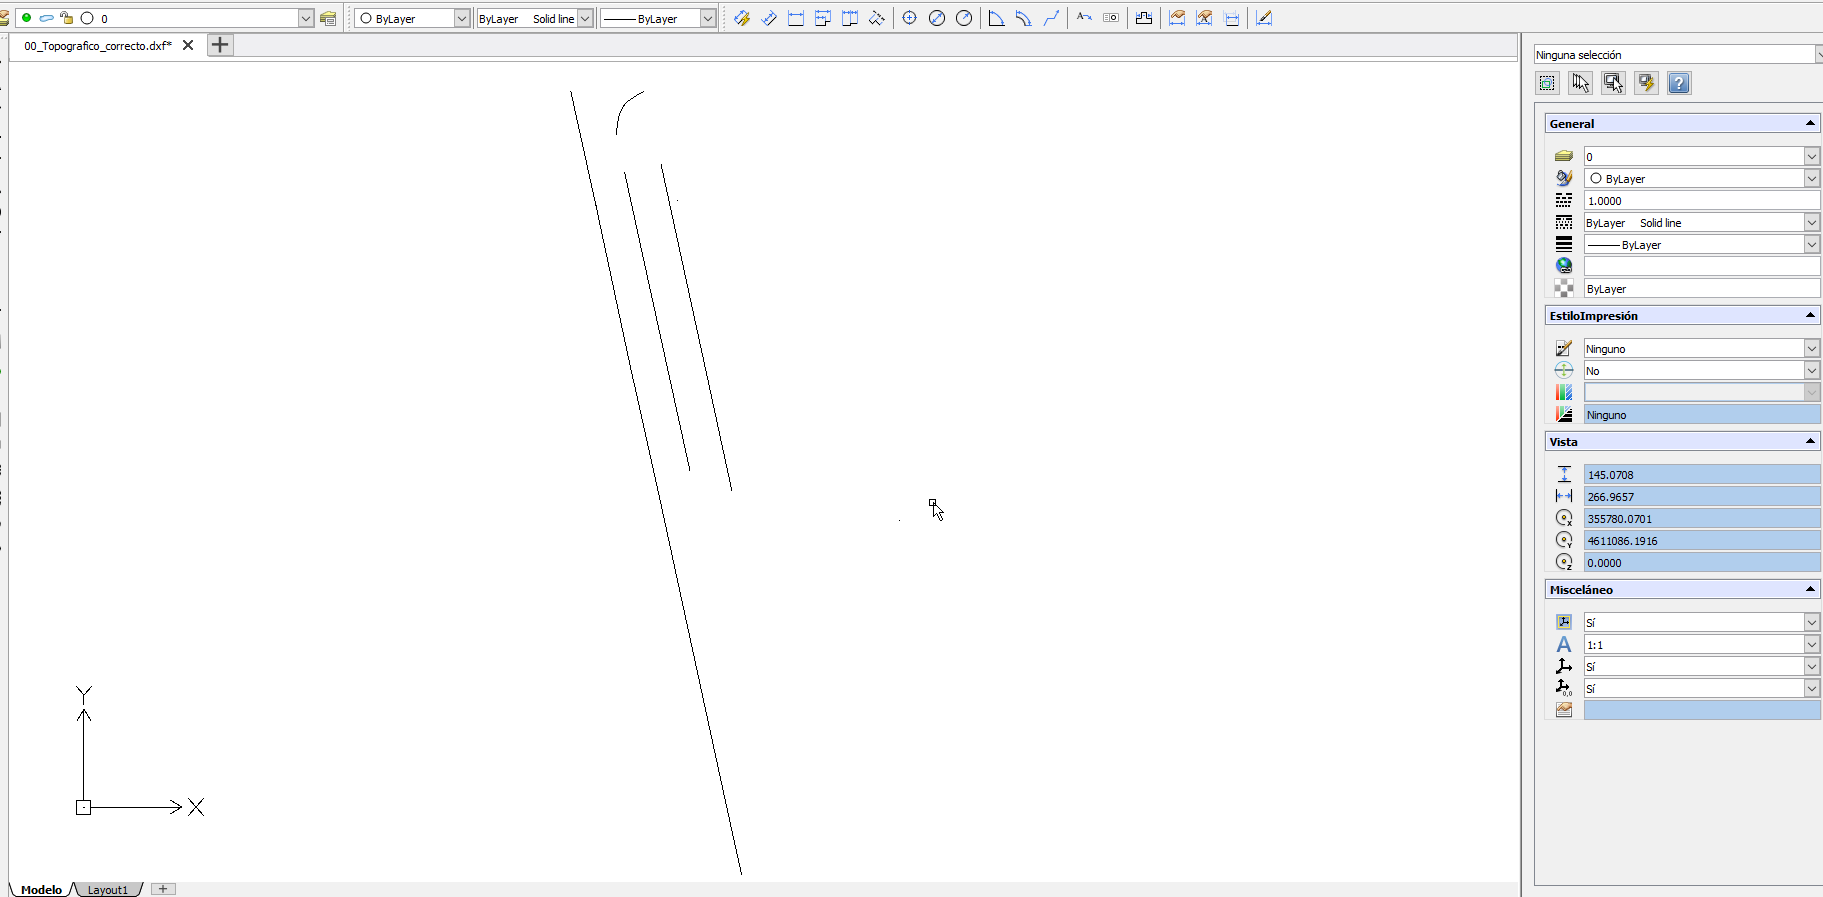
\includegraphics[width=1\textwidth]{proto_1}
	\caption{Dibujo con líneas y \emph{splines}}
	\label{fig:proto_1}
\end{figure}


\subsection{\emph{Sprint} 4 (14/02/2019 - 20/02/2019)}

Una vez acabado el primer prototipo funcional que podía validar un archivo, diferenciar las diferentes lineas y curvas, y generar un archivo DXF, el objetivo de este \emph{sprint} fue comenzar a crear un prototipo  basado en una aplicación Web, utilizando el \emph{micro framework} \texttt{Flask}. Para ello se definieron las siguientes tareas:

\begin{itemize}
\item Formación en \texttt{Flask}: Se consultó la documentación de \texttt{Flask} mencionada en la memoria.

\item Prototipo con \texttt{Flask}: Se creó un prototipo que permitía subir un archivo desde el equipo del usuario al servidor. Se obtuvo un resultado correcto.

\item Procesado del archivo subido y descarga del archivo DXF generado: El prototipo debería validar el archivo subido por el usuario, lo convertiría a DXF, y permitiría descargarlo en su equipo. Se obtuvo un resultado correcto.

\end{itemize}
 
Aquí empezó a trabajar con un entorno virtual creado en \emph{Anaconda}\footnote{\textsl{Anaconda}: \url{https://www.anaconda.com/}} por sugerencia del tutor.


\subsection{\emph{Sprint} 5 (21/02/2019 - 27/02/2019)}

Ya teníamos la aplicación Web funcionando, el siguiente paso sería la validación de usuarios, el uso de una base de datos y a ser posible comenzar a investigar con \emph{Docker} y alojar la base de datos en un contenedor. Para ello se definieron las siguientes tareas:

\begin{itemize}
\item Comenzando con \emph{Docker}: Se consultó la documentación de \\emph{Docker} mencionada en la memoria,y se configuró un contenedor\emph{PostGIS} para alojar la base de datos. También se configuró otro contenedor \emph{PgAdmin4} para poder administrar y ver las modificaciones en la base de datos más fácilmente. También serviría para probar como conectar dos contenedores entre sí.

\item Validación de usuarios: Se implementó la aplicación para que un usuario pudiera logearse y registrarse. Se diseño el modelo de la base datos y la base de datos se crearía automáticamente al arrancar la aplicación. Se utilizaron  las librerías \texttt{SQLAlchemy} y \texttt{Flask-Login} ,mencionadas en la memoria, de las cuales se estudió su documentación. Se obtuvo un resultado correcto.
\end{itemize} 


\subsection{\emph{Sprint} 6 (08/03/2019 - 13/03/2019)}

Este \emph{sprint} se basó en el aprendizaje de \emph{HTML}, formularios y \emph{Bootstrap}. Incluyendo el tratamiento de mensajes \texttt{flash} en \texttt{Flask}.

También se estudió como incorporar un visor en el navegador, para poder visualizar el plano. Se estudiaron varias opciones:

\begin{itemize}
\item Convertir el archivo a formato SVG: Se convirtió el archivo DXF a SVG, con un conversor online\footnote{\textsl{convertio}: \url{https://convertio.co/es/dxf-svg/}}, pero el resultado obtenido no era lo esperado. Se probó con otros conversores siendo el resultado igual de malo, por lo que se descartó esta opción.
  
\item Usar el visor \emph{Three-Dxf}: \emph{Three-Dxf}\footnote{\textsl{Three-Dxf}: \url{https://github.com/gdsestimating/three-dxf}} en un visor en \emph{JavaScript}, para archivos DXF, que se podría incorporar a cualquier aplicación Web. En su documentación indicaba que soportaba los elementos que usábamos en nuestros DXF, como los tipos de lineas, tipos de símbolos, etc. Pero comprobándolo resultó que no era así, daba errores. Conseguía visualizar archivos muy simples, pero no los que necesitábamos en este proyecto.
\end{itemize}

Al final se descartó la idea de que la aplicación tuviera un visor incorporado.

\subsection{\emph{Sprint} 7 (14/03/2019 - 20/03/2019)}

Este \emph{sprint} se basó en implementar funciones que crearan los elementos del archivo DXF. Para ello se definieron las siguientes tareas:

\begin{itemize}
\item Creación de capas: Creación de capas en el DXF, a partir de los códigos del archivo de campo. Hay tres capas que se deberían crear siempre:
\begin{itemize}
	\item \emph{Point:} Capa que deberá contener todos los puntos.
 	\item \emph{Altitude:} Capa que deberá contener la altitud de todos los puntos. 	en forma de texto.
 	\item \emph{Label:}  Capa que deberá contener el código de todos los puntos, en 	forma de texto.
\end{itemize}
Se obtuvo un resultado correcto.

\item Inserción de puntos en el modelo: Se insertan todos los puntos del archivo de campo en el modelo del dibujo. Se dibujan también , los textos correspondientes al código y a la elevación del punto, cada uno en su correspondiente capa, todo ello interpretando la codificación. Se obtuvo un resultado correcto.

\item Creación de circunferencias: Se crearían círculos, a partir de un punto y un radio, y se guardaría en su correspondiente capa, todo ello interpretando la codificación. Se obtuvo un resultado correcto.  

\item Creación de líneas: Se crearían líneas, a partir de una serie de puntos, y se guardarían en su correspondiente capa, todo ello interpretando la codificación. Se obtuvo un resultado correcto. 

\item Creación de cuadrados: Se crearían cuadrados, a partir de dos puntos, y se guardarían en su correspondiente capa, todo ello interpretando la codificación. El cuadrado siempre se dibujaría a la derecha de la alineación definida por estos dos puntos. Se obtuvo un resultado correcto.   

\item Creación de rectángulos: Se crearían rectángulos, a partir de tres puntos, y se guardarían en su correspondiente capa, todo ello interpretando la codificación. Se obtuvo un resultado correcto.   

\item Uso de puntos no medidos en campo: Se utilizarían puntos no medidos en campo para la generación de lineas y se guardarían en su correspondiente capa, todo ello interpretando la codificación. Se obtuvo un resultado correcto.
\end{itemize}

Una vez dibujados los elementos, se mejoró estéticamente el dibujo,modificando el tamaño de los textos y su posición respecto a los puntos.

\subsection{\emph{Sprint} 8 (21/03/2019 - 27/03/2019)}

En este \emph{sprint} se comenzó con la realización de test unitarios, estudiando las diferentes opciones. También como se podría  leer un archivo DXF proporcionado por el usuario, que contuviera símbolos en forma de bloques y una vez , incorporarlos al modelo de dibujo que queríamos generar. Para ello se definieron las siguientes tareas:

\begin{itemize}
\item Estudio de una biblioteca de Python para la realización de los test unitarios : Se consideraron las bibliotecas: \texttt{unittest}\cite{unittest} y \texttt{pytest}\cite{pytest}. La opción elegida fue \texttt{unittest}\, esta biblioteca ya se había usado durante la realización del grado.

\item Comienzo con los test unitarios.

\item Crear una función para cargar un archivo DXF.

\item Crear una función extraer los bloques del archivo DXF.

\item Incorporar los bloques al modelo del dibujo.

\item Asociar cada bloque con cada punto correspondiente, interpretando la codificación.

\end{itemize}

Se obtuvo un resultado correcto.
 
\subsection{\emph{Sprint} 8 (28/03/2019 - 03/04/2019)}

En este \emph{sprint} se comenzó a trabajar con la posibles versiones de CAD que podría generar la aplicación. También se comenzó a trabajar con el archivo de configuración de usuario, definiendo como seria su gramática e implementando un \emph{parser} para poder validarlo. Para ello se definieron las siguientes tareas:

\begin{itemize}
\item Versiones de CAD válidas : Se comprobaría la generación del archivo DXF en diferentes versiones y su validez. 

\item  Definición de gramática para el archivo de configuración de usuario.

\item Carga y validación del archivo de usuario.

\end{itemize}

En este \emph{sprint} se detecta un error en el uso de dos \emph{parsers} que se detalla en la memoria, \textit{Conflicto entre \emph{parsers}.}
 
\subsection{\emph{Sprint} 9 (04/04/2019 - 10/04/2019)}

En este \emph{sprint} se comenzó a trabajar con las sesiones de \texttt{Flask} multiusuario, se continuó con la definición, e implementación de funciones para la gestión del archivo de configuración de usuario y se soluciona el problema de del conflicto entre los dos \emph{parsers}. Para ello se definieron las siguientes tareas:

\begin{itemize}
\item Gestión del archivo de configuración de usuario. 

\item  Problema con el uso de dos \emph{parsers}.

\item Carga y validación del archivo de usuario.

\item Comienzo con las sesiones en \texttt{Flask}.
\end{itemize}

\subsection{\emph{Sprint} 10 (11/04/2019 - 24/04/2019)}

Este \emph{sprint} se consideró más largo, había una semana de vacaciones en medio. Básicamente se basó en completar las funcionalidades Web, el diseño de la Web , y el tratamiento de los mensajes de aviso. Para ello se definieron las siguientes tareas: 
 
\begin{itemize}
\item Añadir funcionalidades a al Web: Añadir o quitar botones, menús, etc.

\item  Mejorar el diseño de la Web: Página de inicio, barra de navegación superior, página de login, etc.

\item Tratamiento de errores: Ver e implementar las distintas formas , en que se presentaran los errores o mensajes de aviso al usuario.

\end{itemize}

Se solucionaron errores como, el surgido al añadir la letra <<ñ>> y la tildes, a la gramática del archivo de configuración (se puede ver la solución en la memoria \textit{ Codificación UTF-8 }). También un error no detectado anteriormente en la función  \texttt{calculate\_azimut\_distance}, con un error de división por 0.
Además se comprobó que la paleta de colores de los programas CAD, no era la habitual (se puede ver la solución en la memoria \textit{ Paleta de colores en CAD})

\subsection{\emph{Sprint} 11 (25/04/2019 - 01/05/2019)}

En este \emph{sprint} y como parte final de la aplicación, el objetivo era que la aplicación se desplegara en \emph{Docker}. En un principio integrar la aplicación \texttt{Flask} y por último ejecutar todos los contenedores a la vez, con el uso de la herramienta \emph{Docker Compose}. Se obtuvo un resultado correcto.

\subsection{\emph{Sprint} 12 (02/05/2019 - 15/05/2019)}

En este \emph{sprint} se tratará de redactar la documentación del proyecto.

\section{Estudio de viabilidad}

\subsection{Viabilidad económica}

En este apartado se analizan los costes del proyecto y también los posibles  beneficios del proyecto en caso de comercializarse.

\subsubsection{Costes}
\textbf{Costes de personal:}

El desarrollo del proyecto, tanto el tiempo empleado en la formación, como la implementación de la aplicación y redactar la documentación
generada, ha sido llevado a cabo por una sola persona durante 476 horas. Considerando 40 horas semanales, hemos trabajado 2.98  meses, por lo que redondeamos a 3 meses de trabajo a tiempo completo. Si consideramos que el trabajo lo ha realizado un programador junior, el salario será el siguiente:

\begin{longtable}[]{@{}lr@{}}
\toprule
\begin{minipage}[b]{0.38\columnwidth}\raggedright\strut
\textbf{Concepto}\strut
\end{minipage} & \begin{minipage}[b]{0.20\columnwidth}\raggedright\strut
\textbf{Coste}\strut
\end{minipage}\tabularnewline
\midrule
\endhead
\begin{minipage}[t]{0.38\columnwidth}\raggedright\strut
Salario mensual neto\strut
\end{minipage} & \begin{minipage}[t]{0.20\columnwidth}\raggedright\strut
1.088.29 \euro{}\strut
\end{minipage}\tabularnewline
\begin{minipage}[t]{0.38\columnwidth}\raggedright\strut
Retención IRPF (15\%)\strut
\end{minipage} & \begin{minipage}[t]{0.20\columnwidth}\raggedright\strut
296.,27 \euro{}\strut
\end{minipage}\tabularnewline
\begin{minipage}[t]{0.38\columnwidth}\raggedright\strut
Seguridad Social (29,9\%)\strut
\end{minipage} & \begin{minipage}[t]{0.20\columnwidth}\raggedright\strut
590,56 \euro{}\strut
\end{minipage}\tabularnewline
\begin{minipage}[t]{0.38\columnwidth}\raggedright\strut
Salario mensual bruto\strut
\end{minipage} & \begin{minipage}[t]{0.20\columnwidth}\raggedright\strut
1.975,12 \euro{}\strut
\end{minipage}\tabularnewline
\midrule
\begin{minipage}[t]{0.38\columnwidth}\raggedright\strut
\textbf{Total 3 meses}\strut
\end{minipage} & \begin{minipage}[t]{0.20\columnwidth}\raggedright\strut
5.925,36 \euro{}\strut
\end{minipage}\tabularnewline
\bottomrule
\caption{Costes de personal.}
\end{longtable}

La retribución\cite{SEG} a la Seguridad Social se ha calculado como un 23,60\% por contingencias comunes, más un 5,50\% por desempleo de tipo general, más un 0,20\% para el Fondo de Garantía Salarial y más un 0,60\% de formación profesional. En total un 29,9\% que se aplica al salario bruto.

El porcentaje de IRPF\cite{IRPF} se ha establecido en el 15\% ya que es el considerado como rendimientos de trabajo para la elaboración de obras científicas.

\textbf{Costes de \emph{hardware} y \emph{software}:}

A continuación se presentan los costes por el emph{hardware} y \emph{software}, utilizado, en el desarrollo del proyecto. Considerando una amortización a 5 años y se ha usado 3 meses.

\begin{longtable}[]{@{}lrr@{}}
\toprule
\begin{minipage}[b]{0.4\columnwidth}\raggedright\strut
\textbf{Concepto}\strut
\end{minipage} & \begin{minipage}[b]{0.18\columnwidth}\raggedright\strut
\textbf{Coste}\strut
\end{minipage} & \begin{minipage}[b]{0.32\columnwidth}\raggedright\strut
\textbf{Coste amortizado}\strut
\end{minipage}\tabularnewline
\midrule
\endhead
\begin{minipage}[t]{0.4\columnwidth}\raggedright\strut
Ordenador personal\strut
\end{minipage} & \begin{minipage}[t]{0.18\columnwidth}\raggedright\strut
1.200 \euro{}\strut
\end{minipage} & \begin{minipage}[t]{0.32\columnwidth}\raggedright\strut
60 \euro{}\strut
\end{minipage}\tabularnewline
\begin{minipage}[t]{0.4\columnwidth}\raggedright\strut
Windows 10 Home\strut
\end{minipage} & \begin{minipage}[t]{0.18\columnwidth}\raggedright\strut
145 \euro{}\strut
\end{minipage} & \begin{minipage}[t]{0.32\columnwidth}\raggedright\strut
7,25 \euro{}\strut
\end{minipage}\tabularnewline
\midrule
\begin{minipage}[t]{0.4\columnwidth}\raggedright\strut
\textbf{Total}\strut
\end{minipage} & \begin{minipage}[t]{0.18\columnwidth}\raggedright\strut
1.345 \euro{}\strut
\end{minipage} & \begin{minipage}[t]{0.32\columnwidth}\raggedright\strut
67,25 \euro{}\strut
\end{minipage}\tabularnewline
\bottomrule
\caption{Costes de \emph{hardware} y \emph{software}.}
\end{longtable}

\textbf{Costes de varios:}

El resto de costes del proyecto son:

\begin{longtable}[]{@{}lr@{}}
\toprule
\begin{minipage}[b]{0.3\columnwidth}\raggedright\strut
\textbf{Concepto}\strut
\end{minipage} & \begin{minipage}[b]{0.18\columnwidth}\raggedright\strut
\textbf{Coste}\strut
\end{minipage}\tabularnewline
\midrule
\endhead
\begin{minipage}[t]{0.3\columnwidth}\raggedright\strut
Alquiler de oficina\strut
\end{minipage} & \begin{minipage}[t]{0.18\columnwidth}\raggedright\strut
250 \euro{}\strut
\end{minipage}\tabularnewline
\begin{minipage}[t]{0.3\columnwidth}\raggedright\strut
Internet\strut
\end{minipage} & \begin{minipage}[t]{0.18\columnwidth}\raggedright\strut
120 \euro{}\strut
\end{minipage}\tabularnewline
\midrule
\begin{minipage}[t]{0.3\columnwidth}\raggedright\strut
\textbf{Total}\strut
\end{minipage} & \begin{minipage}[t]{0.18\columnwidth}\raggedright\strut
370 \euro{}\strut
\end{minipage}\tabularnewline
\bottomrule
\caption{Costes varios.}
\end{longtable}

\textbf{Costes totales:}

El coste total del proyecto es:

\begin{longtable}[]{@{}lr@{}}
\toprule
\begin{minipage}[b]{0.4\columnwidth}\raggedright\strut
\textbf{Concepto}\strut
\end{minipage} & \begin{minipage}[b]{0.22\columnwidth}\raggedright\strut
\textbf{Coste}\strut
\end{minipage}\tabularnewline
\midrule
\endhead
\begin{minipage}[t]{0.4\columnwidth}\raggedright\strut
Personal\strut
\end{minipage} & \begin{minipage}[t]{0.22\columnwidth}\raggedright\strut
5.925,36 \euro{}\strut
\end{minipage}\tabularnewline
\begin{minipage}[t]{0.4\columnwidth}\raggedright\strut
\emph{Hardware \& Software}\strut
\end{minipage} & \begin{minipage}[t]{0.22\columnwidth}\raggedright\strut
67,25 \euro{}\strut
\end{minipage}\tabularnewline
\begin{minipage}[t]{0.4\columnwidth}\raggedright\strut
Varios\strut
\end{minipage} & \begin{minipage}[t]{0.22\columnwidth}\raggedright\strut
370 \euro{}\strut
\end{minipage}\tabularnewline
\midrule
\begin{minipage}[t]{0.4\columnwidth}\raggedright\strut
Total\strut
\end{minipage} & \begin{minipage}[t]{0.22\columnwidth}\raggedright\strut
 6.362,61 \euro{}\strut
\end{minipage}\tabularnewline
\bottomrule
\caption{Costes totales.}
\end{longtable}

\subsubsection{Beneficios}

Se está pensando en distribuir la aplicación comercialmente en un futuro. Un modelo de negocio que se está teniendo en cuenta es, establecer diferentes cuotas por tramos, en función del tamaño de los archivos o del número de puntos a convertir.

Por ejemplo:
\begin{longtable}[]{@{}lr@{}}
\toprule
\begin{minipage}[b]{0.3\columnwidth}\raggedright\strut
\textbf{Número de puntos}\strut
\end{minipage} & \begin{minipage}[b]{0.18\columnwidth}\raggedright\strut
\textbf{Cuota}\strut
\end{minipage}\tabularnewline
\midrule
\endhead
\begin{minipage}[t]{0.3\columnwidth}\raggedright\strut
10.000 \strut
\end{minipage} & \begin{minipage}[t]{0.18\columnwidth}\raggedright\strut
10 \euro{}/mes \strut
\end{minipage}\tabularnewline
\begin{minipage}[t]{0.3\columnwidth}\raggedright\strut
30.000 \strut
\end{minipage} & \begin{minipage}[t]{0.18\columnwidth}\raggedright\strut
20 \euro{}/mes \strut
\end{minipage}\tabularnewline
\begin{minipage}[t]{0.3\columnwidth}\raggedright\strut
Sin Límite \strut
\end{minipage} & \begin{minipage}[t]{0.18\columnwidth}\raggedright\strut
40 \euro{}/mes \strut
\end{minipage}\tabularnewline
\bottomrule
\caption{Tipos de suscripciones y cuotas}
\end{longtable}

Añadiendo nuevas funcionalidades, se estudiarán otros parámetros en el modelo de negocio como por ejemplo, si el usuario desea:
\begin{itemize}
\item Imprimir el plano.
\item Almacenar en la aplicación una base de datos con símbolos.
\item Unir varios archivos.
\item Modificar la escala y el formato del plano.
\item ...
\end{itemize}

En este caso la idea sería ofrecer paquetes con diferentes funcionalidades a diferentes precios, por ejemplo:

\begin{itemize}
\item Paquete básico: Conversión de ficheros.
\item Paquete intermedio: Conversión de ficheros, cambios de escalas y formatos.
\item Paquete avanzado: Conversión de ficheros, cambios de escalas y formatos, impresión de archivos.
\item Paquete completo: Todas las opciones.
\end{itemize}

Podría existir una funcionalidad gratuita, que permitiera visualizar el archivo, sin permitir nada más, para atraer posibles clientes.



\subsection{Viabilidad legal}
